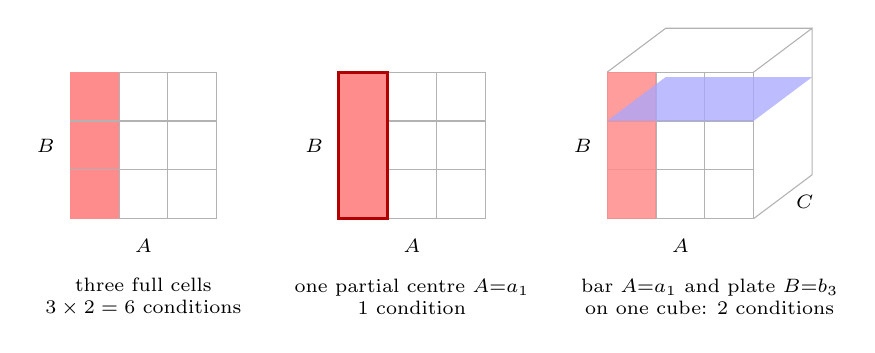
\begin{tikzpicture}[scale=0.62,every node/.style={font=\scriptsize}]
\begin{scope}
\draw[step=1,gray!60] (0,0) grid (3,3);
\fill[red!45] (0,0) rectangle (1,3); \draw[gray!60] (0,1)--(1,1) (0,2)--(1,2);
\node at (1.5,-0.55) {$A$}; \node at (-0.5,1.5) {$B$};
\node[align=center] at (1.5,-1.6) {three full cells\\ $3\times2=6$ conditions};
\end{scope}
\begin{scope}[xshift=5.5cm]
\draw[step=1,gray!60] (0,0) grid (3,3);
\fill[red!45] (0,0) rectangle (1,3); \draw[red!70!black,very thick] (0,0) rectangle (1,3);
\node at (1.5,-0.55) {$A$}; \node at (-0.5,1.5) {$B$};
\node[align=center] at (1.5,-1.6) {one partial centre $A{=}a_1$\\ $1$ condition};
\end{scope}
\begin{scope}[xshift=11cm]
\draw[gray!60] (0,0) grid (3,3);
\draw[gray!60] (3,0)--(4.2,0.9)--(4.2,3.9)--(3,3); \draw[gray!60] (0,3)--(1.2,3.9)--(4.2,3.9);
\fill[red!45,opacity=.85] (0,0) rectangle (1,3);
\fill[blue!35,opacity=.75] (0,2)--(3,2)--(4.2,2.9)--(1.2,2.9)--cycle;
\node at (1.5,-0.55) {$A$}; \node at (-0.5,1.5) {$B$}; \node at (4.05,0.35) {$C$};
\node[align=center] at (2.1,-1.6) {bar $A{=}a_1$ and plate $B{=}b_3$\\ on one cube: $2$ conditions};
\end{scope}
\end{tikzpicture}
